\documentclass[12pt,a4paper]{article}	%only 10 to 12 working in article
\usepackage[left=2cm, right=2cm, top=1cm]{geometry}

\usepackage{upgreek}
%type greek letter command between $' '$ !!

\usepackage{graphicx}
\usepackage{subcaption}
%packages for inserting image


\title{Introduction to the Experiment}
\date{\vspace{-5ex}}	%to skip printing the dat in the title

\begin{document}
\maketitle
\thispagestyle{empty}	%To supress the printing of page number
\large
The purpose of torsion testing usually parallels that of uniaxial tension tests. From the experiment, the shear elastic modulus (G), shear proportional stress ($\tau$\textsubscript{p}), shear yield stress ($\tau$\textsubscript{y}), and the Stress-Strain behavior in general, can be obtained. However, in contrast to uniaxial tension tests, the stresses are not distributed uniformly over the cross section. \\

Torsion loading results in twisting of one section of a body with respect to a contiguous section. During the test the angle of twist $\phi$ and the applied torque T are measured as the test proceeds. For a circular cross-section, in the absence of the other loads, pure shear stress state exists at each point. Torsional elastic shear stresses vary linearly from zero at the axis of twist to a maximum at the extreme fibers. Thus, in a solid circular bar, when the surface fibers reach the yield shear stress they are, in a sense, supported by elastic interior fibers. Consequently, the elastic resistance of the remainder of the section masks the effect of yielding of the surface fibers during their early stage of yielding. Usually, it is not until considerable yielding has taken place that any noticeable effect of nonlinearity is apparent using a simple mechanical troptometer to measure the angle of twist $\phi$ \\

To test the material in torsion the proper test procedure is needed. It involves mounting a shaft into the testing machine, applying torque incrementally and measuring both the applied torque and the corresponding angle of twist. Using the appropriate formulae, relationships and the measured dimensions, we can determine the shear stress and shear strain on the shaft. Then, one can plot the torque vs. angle of twist, and shear stress vs. shear strain from which one can find the material properties previously mentioned. \\

\textbf{Apparatus} other than testing specimen:
\begin{enumerate}
\item Caliper 
\item Troptometer 
\item Torsion testing machine 
\item Measuring tape
\end{enumerate}

	\thispagestyle{empty}	%To supress the printing of page number
\begin{figure}[h!]
	\centering
		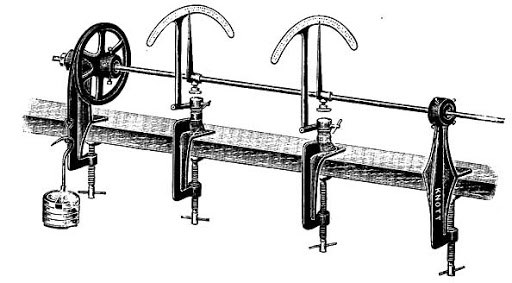
\includegraphics[width=\linewidth]{Torsion Apparatus Old.jpg}
		\caption{Torsion Apparatus}
\end{figure}

\begin{figure}[h!]
	\centering
	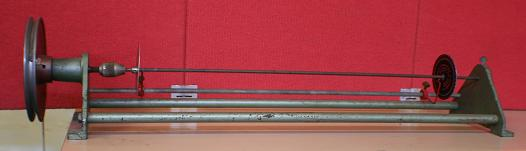
\includegraphics[width=\linewidth]{Problem Statement Setup.jpg}
	\caption{Torsion Apparatus Setup}
\end{figure}

\begin{figure}[h!]
	\centering
\begin{subfigure}[b]{4.2cm}
	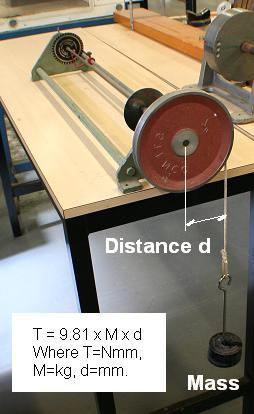
\includegraphics[width=\linewidth]{Problem Statement Setup2.jpg}
	\caption{Lever}
\end{subfigure} \hspace{10mm}%to add space 
\begin{subfigure}[b]{8.5cm}
	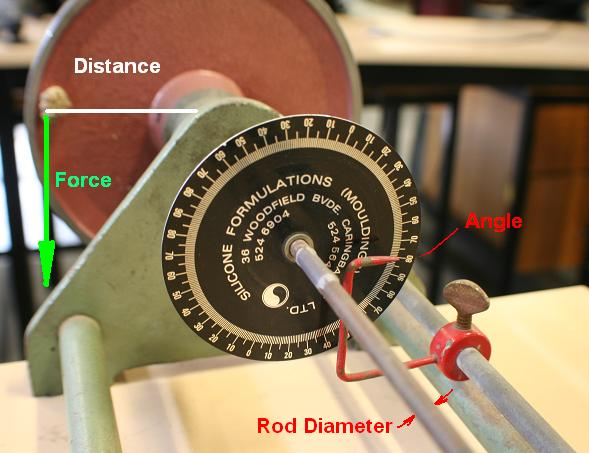
\includegraphics[width=\linewidth]{Problem Statement Setup3.jpg}
	\caption{Deflection Indicator}
\end{subfigure}
\end{figure}


\break

\textbf{The assumptions made in this experiment include the following:}
\begin{enumerate}
\item The torque is applied along the center of axis of the shaft. 
\item The material is tested at steady state (absence of strain rate effects). 
\item Plane sections remain plane after twisting (the circular section conforms to this condition). \\
\end{enumerate}

\textbf{Test Procedure:}
\begin{enumerate}
\item Measure the diameter of the test specimen using the caliper (take an average of 5 measurements). 
\item Slide the shaft into the Torsion Test Apparatus and tighten down the two fastening screws to the shaft.  
\item Clean the clamps used to hold the shaft in place. \item Insert the shaft into the right clamps. Tighten the clamp ensuring that the grip is very tight.
\item Adjust the Torsion Test Apparatus to the correct position pointing at 0 degree initially. 
\item Measure the length between the Torsion Test Apparatus clamps Lt using the tape measure. This length is the effective length of the rod between which the Torsion takes place 
\item Add weights to the lever gradually and note down the Apparatus reading of the deflection
\item After loading the lever,unload it by taking the masses off one by one and note down the Apparatus reading of the deflection.
\item Repeat this cycle 20 times to obtain sufficient data to  find a good estimate of the Shear Modulus\\
\item Calculate the Stress and Strain with the recorded data and plot a Shear Stress vs Shear Strain Curve.
\textbf{The slope of the Shear Stress vs Shear Strain curve gives the value of the Shear Modulus G}\\
\end{enumerate}
\thispagestyle{empty}	%To supress the printing of page number

\textbf{Results :}\\
Experimental Shear Modulus of Aluminium 6061 : 20.2659 $\pm$ 3.2629 GPa\\
Published Shear Modulus of Aluminium 6061 : 26 GPa\\

\break
\textbf{Discussion:}\\
As we can see the Experimental value is less than the Published value. A part of this can be attributed to the fact that since we can not measure angles beyond a certain precision,we have taken a larger range of Strain to calculate the Shear Modulus.This means that the values that are obtained are not strictly confined to the proportionality limit and may exceed it.\\

Beyond the Proportionality Limit the Stress does not increase linearly with Strain and slope of Stress vs Strain graph decreases. Thus when we apply a Linear Fit, the slop of the Best Fit line is less than the slope of the Stress vs Strain graph in the Proportionality Limit.
Due to this reason we obtain a value less than the Published value and not more than it.\\


Another observation we made was that the Precision of the Data given to us was higher than the Precision of the Torsion Apparatus.This suggests the use of a more precise apparatus than mentioned\\

\textbf{Conclusion:}
\begin{itemize}
\item We understood that Modulus of rigidity is the coefficient of the elasticity for a shearing force, it measure the stiffness of the particular materials in torsion test. 
\item Different type of material will have different elastic limit. The higher value of modulus of rigidity, G , the higher the torsion stiffness of material .
\item If the material exceeds the elastic limit,permanent deformation will be occurring. On exceeding the proportionality limit the objective of this experiment will be defied.
\item We learnt how Torsion Test can be used to calculate the Shear Modulus of a Material.
\item Learning about the Errors that might persist during the Torsion Test and how to minimize them
\item Using tools with limited technology and precision,the Torsion Test gives a decent esitmate of the Shear Modulus of a material

\end{itemize}

\thispagestyle{empty}	%To supress the printing of page number
\end{document}
